% Add abstract etc?

\section{Introduction}
% This is why we want it.
Program instrumentation is a technique used in many and diverse areas.
Instrumentation is often added to programs in order to investigate performance
aspects of the applications~\cite{paradyn95,etch} as a complement to
statistical profiling such as gprof~\cite{graham83gprof}, Intel
VTune~\cite{wolf99vtune}, or the Digital Continuous Profiling
framework~\cite{anderson97cpw}. Instrumentation is also useful in many
other areas not directly related to performance analysis, for instance call
graph tracing~\cite{steignerwilke2003verstehen}, path
profiling~\cite{ball96efficient}, reversible
debugging~\cite{chen2001reversible}, code coverage analysis, and
security~\cite{miller01pib}.

% They are hard to use
Often, instrumentation is added manually by annotating the source code with
instrumentation points. This task, however, is time-consuming, repetitive and
error-prone, and it is both tied to the high-level language and access to
source code. Over the years, there has therefore been a number of proposals to
alleviate this situation. Today, there exists several libraries, e.g.,
ARM~\cite{armAPI} and PAPI~\cite{london2001papi}, which allows code-reuse for
the instrumentation.  There are also packages that provide graphical
interfaces to select instrumentation-points and several tools for patching
program binaries or relocatable object files~\cite{paradyn95,eel}.

%\emph{What should an instrumentation package fulfil}: Easy to use (no code
%changes, good if application can be patched directly), low overhead, high
%detail, reproducability.
Another problem with program instrumentation is program behavior perturbations
caused by the
instrumentation~\cite{maloney1992instrumentation,moseley2003checking}.
Regardless of how instrumentation is implemented, it always adds extra work
for the program by affecting compiler optimizations (changed register
allocation, reduced inlining possibilities etc.), altering the data reference
patterns, and changing the execution flow.  Taken together, these
perturbations can cause the instrumented program to exhibit a substantially
different behavior than the uninstrumented program.  This problem is
especially severe for performance instrumentation since the instrumented
program should accurately reflect the uninstrumented program, and it is
therefore important to measure and minimize the instrumentation overhead. The
measurement itself can also be a problem, however. Although it is easy to
measure the aggregate overhead of instrumenting a program, observing the
detailed behavior of the instrumentation is harder since any performance
measurement affects the program execution. Taken together, these problems lead
us to we believe that it is important to explore optimizations for
instrumentation, especially for frequently performed operations.
% It is hard to measure instrumentation perturbation

In this paper, we present the LOPI (LOw Perturbation Instrumentation)
framework that provides a generic and easily used framework for instrumenting
programs. In LOPI, we try to optimize for common instrumentation patterns in
order to provide low perturbation on the program behavior. LOPI rewrites
binary ELF-files for GNU/Linux on the IA-32 architecture in order to
instrument an application.  The current implementation instruments function
entry and exit, but the approach is expandable to instrument most points in
the code.

We provide measurements of the instrumentation perturbation using both real
hardware and full-system simulations of seven SPEC CPU2000 benchmarks.  We
compare the LOPI framework to Dyninst\cite{buck00dyninst} and regular
source-based instrumentation.  We find that source-based instrumentation
usually has the lowest instrumentation overhead, on average executing 13\%
more instructions (5\% inlined) for the studied applications, but with more
tedious work for instrumenting the code.  Comparing LOPI and Dyninst we find
that LOPI has lower instruction overhead then Dyninst, on average 36\%
instruction overhead compared to 49\% for Dyninst.  Comparing the total
execution times, we find that source-based instrumentation has 6\% overhead,
LOPI has 22\% overhead, and Dyninst 28\% overhead as compared to an
uninstrumented application.

% In addition, our results show that LOPI generates fewer additional
%cache misses than Dyninst. For example, LOPI generates 57\% more misses in the
%first-level instruction cache, while Dyninst generates 87\% more misses on
%average.

% We have a technique that gives lower instrumentation
% Present some of the main results

The rest of the paper is organized as follows. In Section~\ref{sec:lopi:background}
we provide an overview of program instrumentation, which is followed by an
introduction of the LOPI framework in Section~\ref{sec:lopi:lopi}. In
Section~\ref{sec:lopi:methodology} we present the measurement methodology and in
Section~\ref{sec:lopi:measurements} we provide the measurement results.  Finally,
we discuss related work in Section~\ref{sec:lopi:related_work} and conclude our
findings in Section~\ref{sec:lopi:conclusion}.

\section{Background}
\label{sec:lopi:background}

\subsection{Instrumentation approaches}
Instrumentation packages can be grouped into three broad categories with
different characteristics: \emph{source-based instrumentation}, \emph{binary
  rewriting}, and \emph{memory image rewriting}.  There are some special
cases, for instance instrumentation at the assembly level, but these can
normally be generalized into one of the above (assembly-level instrumentation
is similar to binary rewriting except that it avoids some issues with
relocatable code). Also, some completely different approaches exist.
Valgrind~\cite{valgrind}, for instance, allows instrumentation of unmodified
programs. Valgrind works by running programs in a virtual machine, translating
IA-32 binary code to a intermediate language, applying instrumentation, and
then translated back to IA-32 code again. Valgrind allows instrumenting
unmodified programs, but also imposes a high runtime overhead due to the code
translation. Another approach is to run the application in a simulator, which
gives no perturbation to the actual application, but has issues with accuracy
and speed. Next, we will briefly describe the different approaches.

\begin{enumerate}
\item \textbf{Source-based instrumentation}: Source-based instrumentation
  works by inserting instrumentation calls as statements in the application
  source code. This allows the compiler to optimize the instrumented code, but
  it also inherently produces a different behavior compared to the
  non-instrumented code because of disturbed register allocation, inlining,
  etc. Further, this approach is dependent on the high-level implementation
  language as well as direct access to the source code.

  This category encompasses both libraries for instrumentation, i.e., where
  instrumentation is inserted manually into the source
  code~\cite{london2001papi}, mixed solutions~\cite{garcia2003PET}, and tools
  with source-to-source conversion from a graphical
  interface~\cite{steigner2001cosmos}.

\item \textbf{Binary rewriting}: By patching the executable or the relocatable
  files, the high-level source code of the application can remain untouched.
  This prevents the compiler from optimizing the instrumentation code in the
  context of the application source code, but this should also give a closer
  correspondence to the uninstrumented application. This approach is also
  independent of the high-level language of the application and can in
  principle be used on applications for which the source code is unavailable.

  Many instrumentation packages work this way, for instance ATOM~\cite{atom}
  and EEL~\cite{eel} for UNIX-based systems, Etch~\cite{etch} and
  PatchWrx~\cite{casmira98tcw} for Windows NT systems, and the LOPI
  framework presented here.

\item \textbf{Memory image rewriting} A final approach is to patch the
  application in-core, i.e., after the program has been loaded into memory.
  This approach, used by Dyninst~\cite{buck00dyninst, paradyn95}, allows
  instrumentation to be added to and removed from the program during runtime.
  The characteristics is similar to binary rewriting but memory image
  rewriting allows instrumentation to be dynamically removed when it is no
  longer needed, which can reduce unnecessary overhead.

  Memory image rewriting also adds some other interesting possibilities. Some
  programs, for instance operating system kernels cannot readily be restarted
  in order to have the instrumentation take effect. For these cases, memory
  image rewriting provides the only realistic alternative, and it has also
  been used for instrumentation of the Solaris~\cite{tamches1999kerninst} and
  Linux~\cite{pearce02gdi} kernels.
\end{enumerate}

Each of these methods will cause perturbation to the application. Next we
present an introduction to the various types of perturbation caused by
instrumentation.

\begin{figure*}[t]
  \begin{center}
    \epsfig{width=1.0\linewidth, file=figures/lopi/lopi_overview}
  \end{center}
  \caption[The instrumentation process]{Overview of the instrumentation
    process. The functions and the files to instrument are given on the
    command line.}
  \label{fig:lopi:lipo_overview}
\end{figure*}

\subsection{Instrumentation perturbation}
Instrumentation perturbation is heavily dependent on the type of
instrumentation applied. For performance instrumentation, the instrumentation
might read a set of of hardware performance counters whereas call graph
tracing requires significantly more complex
operations~\cite{steignerwilke2003verstehen}. Some parts are very common
however. At the very basic end, instrumentation always causes more
instructions to be executed, accesses more data in the memory, and can also
cause register spills. Further, there might be kernel invocations, device
access or inter-process communication. The perturbation also varies over
different phases of the program execution:

\begin{itemize}
\item \textbf{Initialization}: Most instrumentation packages have some sort of
  initialization phase. This can include, e.g., the initialization of hardware
  performance counters, creation of data structures, or memory image patching.
  This part can sometimes be very expensive, but is a one-time event.
\item \textbf{Startup-phase}: During the first invocations of the instrumented
  code, the system will run with cold caches and need to bring the code and
  data into the caches.
\item \textbf{Execution}: During the execution of the program, the
  instrumentation adds latency because more instructions are executed,
  increased cache pressure, and (potentially) extra kernel invocations.
\item \textbf{End}: When the program ends, or the instrumentation is removed,
  the instrumentation package usually performs some cleanup operations (for
  instance freeing allocated memory, storing collected data on disk etc.).
  Like the initialization-phase, this is potentially expensive but normally
  has small effects on long-running programs.
\end{itemize}

For the execution phase, there are also some indirect effects on the execution
that can arise from instrumentation. For instance, the addresses of data or
executed instructions might change as a side-effect of instrumentation (this
is especially likely with source instrumentation). The changed addresses can
cause data or code to be aligned differently with respect to cache-lines, and
also in some cases (albeit unusual) change actual program
behavior~\cite{moseley2003checking}. In the LOPI framework, we have tried to
minimize these effects by a number of optimizations, which are described in the
next section.

\section{The LOPI instrumentation framework}
\label{sec:lopi:lopi}
We have implemented an instrumentation package that tries to provide low and
predictable overhead and still provide an easy interface to users.  The
framework uses the binary rewriting approach, although the ideas are
applicable to memory rewriting (such as used by Dyninst) as well. Although we
currently focus on function entry and exit, the approach is possible to
combine with current methods for instrumentation at arbitrary points (still
keeping the optimized entry/exit techniques). We have developed two types of
performance instrumentations for LOPI, one utilizing the PAPI cross-platform
front-end to performance counters~\cite{london2001papi} and one simple
implementation measuring the processor cycle counter with the \texttt{rdtsc}
instruction.

% FIXME: Add some comments on multithreading here

The process of instrumenting a program with the LOPI framework is shown in
Figure~\ref{fig:lopi:lipo_overview}. Using the LOPI framework adds one step in the
compile process - running the LOPI executable after the relocatable files have
been produced. The relocatable ELF-files are then linked with a library
produced by LOPI at runtime, which contains stubs and the user-implemented
instrumentation. Note that selecting the instrumentation points is done
outside the LOPI framework in order to keep the framework general enough to
support different kinds of instrumentation.

\begin{figure*}[htb]
  \begin{center}
    \epsfig{width=1.0\linewidth, file=figures/lopi/non_inst_call}
  \end{center}
  \caption{A non-instrumented function call.}
  \label{fig:lopi:non_inst_call}
\end{figure*}

\begin{figure*}[htb]
  \begin{center}
    \epsfig{width=1.0\linewidth, file=figures/lopi/instrumented_call}
  \end{center}
  \caption[An instrumented function call]{A function call
    instrumented with our approach.}
  \label{fig:lopi:instrumented_call}
\end{figure*}

\begin{figure*}[htb]
  \begin{center}
    \epsfig{width=1.0\linewidth, file=figures/lopi/instrumented_return}
  \end{center}
  \caption[An instrumented function return]{An instrumented function return.}
  \label{fig:lopi:instrumented_return}
\end{figure*}

Before going into details of the operation, we will first briefly
describe the (GCC) calling convention for the IA-32 architecture.
Figure~\ref{fig:lopi:non_inst_call} shows how \emph{caller} calls the
non-instrumented function \emph{callee}.  On IA-32, the
\texttt{call}-instruction pushes the return address to the stack before
switching to the function. On returning with \texttt{ret}, the instruction
pointer is popped from the top of the stack. The IA-32 calling convention
specifies that registers \texttt{\%ebx}, \texttt{\%edi}, \texttt{\%esi}, and
\texttt{\%ebp} are callee-saved, whereas \texttt{\%eax}, \texttt{\%ecx} and
\texttt{\%edx} are caller-saved. Parameters are passed on the stack and the
return value is passed in the \texttt{\%eax} register. The function prologue
shown initializes the function stack frame.

A function entry instrumented with the LOPI framework is shown, somewhat
simplified, in Figure~\ref{fig:lopi:instrumented_call}. When the program execution
reaches an instrumentation point, our library performs a four step operation.
The sequence of events is shown in the figure and described below.

\begin{enumerate}
\item \texttt{enter\_stub} is called (from \emph{callee}) by the overwritten
  function prologue (which was replaced by the instrumentation). The
  \texttt{call}-instruction is immediately followed by an identifier for the
  function (\texttt{func\_nr}). The function identifier defaults to a 8-bit
  value, but if more than 256 functions are instrumented this can be extended
  to a 16- or 32-bit value at instrumentation time (this has not yet been
  implemented, but the extension is simple to make).

\item \texttt{enter\_stub} (shown in Figure~\ref{fig:lopi:instrumented_call}) reads
  the function identifier (which is located at the return address, i.e., in the
  \emph{callee}-prologue). Then, the enter stub calls
  \texttt{instr\_func\_enter}, which is common for all instrumented function
  entries.

\begin{figure}[htb]
  \begin{center}
    \begin{pseudocode}
         \STRUCT{ret\_frame\_t}
          func\_t~~*p\_func \\
          long~~~~~ret\_addr \\
          \COMMENT{For icache/dcache conflict reduction}
          uint8\_t~~padding0[XX] \\
          uint8\_t~~program[16]\\
          uint8\_t~~padding1[XX] \\
          ...
        \ENDSTRUCT
        \\
        ret\_frame\_t ret\_frames[]
        \\
        \\
        \FUNC{instr\_func\_enter}{func\_nr, ret\_addr}
          \COMMENT{Setup return frame}
          ret\_frame = pop\_ret\_frame()\\
          ret\_frame.func = funcs[func\_nr]\\
          ret\_frame.ret\_addr = ret\_addr\\
          *ret\_addr = ret\_frame.program\\
          \\
          \COMMENT{Perform the instrumentation}
          do\_enter\_func(func)
        \ENDFUNC
      \end{pseudocode}
    \end{center}
    \caption{Pseudo code for the \texttt{instr\_func\_enter}-function.}
    \label{fig:lopi:instr_func_entry_code}
\end{figure}

\item The \texttt{instr\_func\_enter}-function, implemented in C (pseudo code
  in Figure~\ref{fig:lopi:instr_func_entry_code}), sets up a return frame to
  instrument the function return. \texttt{inst\_func\_enter} thereafter
  performs the actual instrumentation operation for function entries, which is
  implemented by the user of the instrumentation library and can be inlined.
  Access to the return frames is protected by a spinlock for multithreaded
  programs on SMPs.

\item After returning to the enter stub, the overwritten instructions of the
  function prologue are executed and the control returns to the function
  prologue (after the overwritten instructions).
\end{enumerate}

There are some special cases for instrumenting function entry points, which
suggest separate handling. First, we detect the common function prologue where
the frame pointer (the \texttt{\%ebp} register) is stored and a new stack
frame is setup. This code sequence only varies with a constant, which gives
the size of the new stack frame, and can therefore easily be represented by a
common stub.

\begin{pseudocode}
  pushl~\%ebp~~~~~~~\COMMENT{Save the old frame pointer}
  movl~~\%esp,~\%ebp~\COMMENT{Set the start of the new frame}
  subl~~~\$XX,~\%esp~\COMMENT{Allocate stack space}
\end{pseudocode}

In the seven SPEC CPU2000 benchmarks we used (see
Section~\ref{sec:lopi:methodology}), almost 80\% of the function prologues had this
pattern. This function prologue is represented with a special stub that stores
the stack size \texttt{XX}.  In the rare case that the function prologue is
smaller than 6 bytes (the size of the call-instruction plus the function
identifier) and the first basic block at the same time contains a branch
target within the first 6 bytes, patching the function prologue is unsafe
because the target instruction is overwritten.  LOPI will detect and mark such
areas as unavailable for instrumentation, although this functionality is only
sketched in the prototype implementation.

Function returns are instrumented lazily with the return frames set up in
\texttt{instr\_func\_enter}, i.e., without patching or adding source lines to
the program. The return frame is a data structure with the original return
address (i.e., back to \emph{caller} in this case), which also contains a
machine code stub, copied to the structure at startup. The padding is needed
since the return frame is accessed both as data and executed as code. Without
the padding, the cache block (the stub is only 16 bytes) would ping-pong
between the data and the instruction cache, degrading performance.
The machine code stub acts as a trampoline for the function return
instrumentation. The logic is as follows (refer to
Figure~\ref{fig:lopi:instrumented_return}):

\begin{enumerate}
\item The \emph{callee} function returns with the \texttt{ret} instruction
  (i.e., exactly as without instrumentation). Since the return address was
  overwritten it will return to the return frame stub setup in
  \texttt{instr\_func\_enter}.

\item The return frame stub calls \texttt{instr\_func\_leave}. Since the
  position of the return frame (and thus the return stub) is unknown at
  compile-time, we need to do a register-relative call to
  \texttt{instr\_func\_leave} (not shown in the figure).

\item \texttt{instr\_func\_leave} performs the instrumentation on function
  exit (again specified by the user of the library), deallocates the return
  frame, and returns the original return address (i.e., to \emph{caller} in
  this example). The pseudo code is shown in
  Figure~\ref{fig:lopi:instr_func_leave_code}.
\end{enumerate}

For functions which modify the return address themselves, this optimization is
unsafe, and a revert to a more traditional return instrumentation is needed.
We reduce the perturbation of the instrumented application in a number of ways
both during the program patching and during runtime:

\begin{figure}
  \begin{center}
    \begin{pseudocode}
      \FUNC{instr\_func\_leave}{}
        \COMMENT{This code is contained in the ret\_frame}
        ret\_frame = [return address]-XX \\
        \COMMENT{Perform the instrumentation}
        do\_leave\_func(ret\_frame.func) \\
        \\
        push\_ret\_frame(ret\_frame) \\
        \COMMENT{Found in the ret\_frame}
        \RETURN{[original return address]}
      \ENDFUNC
    \end{pseudocode}
  \end{center}
  \caption{Pseudo code for the \texttt{instr\_func\_leave}-function.}
  \label{fig:lopi:instr_func_leave_code}
\end{figure}

\begin{table*}[thb]
  \begin{center}
    \caption[Benchmark description]{Description of the SPEC CPU2000 benchmarks
      used in this study.}
  \label{tab:lopi:benchmarks}
  \begin{tabular}{|l|l|l|}
       \hline
       \hline
       Benchmark  & Description & Data set size \\
       \hline
       \hline
       164.gzip   & Compression & lgred.log \\
       \hline
       176.gcc    & Compiler & smred.c-iterate.i \\
       \hline
       181.mcf    & Combinatorial optimization & lgred.in \\
       \hline
       183.equake & Simulation of seismic wave propagation & lgred.in \\
       \hline
       197.parser & Grammar analysis & lgred.in \\
       \hline
       256.bzip2   & Compression & lgred.graphic \\
       \hline
       300.twolf   & CAD, Placement and global routing & lgred \\
       \hline
       \hline
  \end{tabular}
  \end{center}
\end{table*}

\begin{enumerate}
\item \textbf{Inlined function identifiers}. The function identifier (shown in
  Figure~\ref{fig:lopi:instrumented_call}) is placed directly in the instrumented
  code in order to avoid the need for calling separate stubs for every
  instrumentation point. The function identifier also allows us to lookup
  meta data for the instrumentation point by using it as a vector index
  instead of performing an expensive hash table lookup.
\item \textbf{Code reuse}. A call-stub is shared for every instrumentation
  point with the same overwritten instructions. Also, the stubs are kept as
  short of possible with most of the logic in the generic enter and exit
  functions.
\item \textbf{Optimize for common cases}. We use a special stub for the common
  stack frame setup as explained in Section~\ref{sec:lopi:lopi}. This helps down the
  i-cache miss rate by reducing the number of instrumentation stubs.

\item \textbf{Register saving}. Our entry stubs does not store any registers
  for the function entries since we do not use any callee-saved registers in
  the stub. The return frame saves the \texttt{\%eax} register since this is
  used for return values on IA-32.
\item \textbf{Data reuse}. The return frames are allocated in a stack-based scheme
  where the most recently used return frame is reused first.
\end{enumerate}

The pollution of the instruction cache is limited by the number of function
call stubs used in the instrumentation and the number of return frames used.
The number of active return frames at a given point of time is equal to the
current nesting depth of the instrumented functions, in most cases a fairly
low number (the worst case occurs with deep recursion).

Taken together, these optimizations significantly reduce the overhead
of instrumentation. Further, since the call-stubs are aggressively reused, we
expect the perturbation to be more predictable since less code is added to the
program. The next section presents measurements comparing our approach to the
Dyninst tool and basic source-based instrumentation.

\section{Measurement methodology}
\label{sec:lopi:methodology}
% Why simics?
For our measurements, we have used both real hardware and the Simics
full-system simulator~\cite{simics}.  The machine we used is a Pentium III
system running Linux, with a 1~GHz processor and 256 MB RAM. We use
the hardware performance counters available on the Pentium III (through the
PAPI~\cite{london2001papi} library) to capture the measures presented in
Table~\ref{tab:lopi:agg_overhead}, e.g., the number of instructions and cache
misses.

\begin{figure*}[htb]
  \begin{center}
    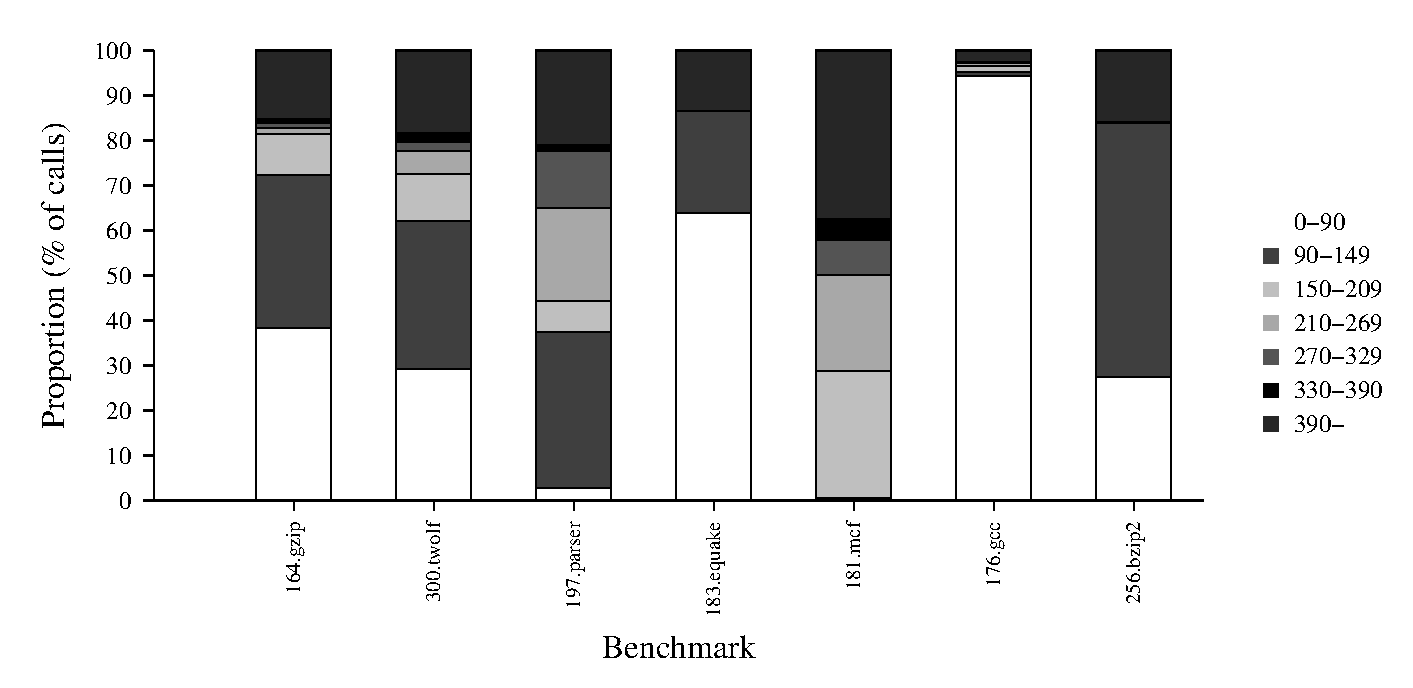
\epsfig{width=1.07\linewidth, file=data/lopi/eps/1_func_avgs_STACKED_reduced}
  \end{center}
  \caption[Cycles per function call]{Cycles per function call on a subset of
    the SPEC CPU2000 benchmarks.}
  \label{fig:lopi:function_averages}
\end{figure*}

As for our simulations, we simulate a complete Pentium III system with caches
running a real operating system for performing the instrumentation
measurements. The simulated system has 16 KB, 4-way set-associative,
first-level data and instruction caches, and a unified 512KB, 8-way
set-associative, second-level cache. Simics allows us to create a complete
non-intrusive measurement of the application execution, both for instrumented
and non-instrumented applications. We can therefore isolate the impact of
instrumentation from the application traces. We use Simics to provide detailed
execution characteristics which were not possible to capture on real hardware,
i.e., the figures in Figure~\ref{fig:lopi:exec_profile}.

%A drawback with using
%Simics is that (at the time of our measurements) it did not provide exact
%instruction timing on IA-32, which means that the cycle count will differ from
%measurements on real hardware.

% How is the simulated tracing done
% 80%..
We ran tests with seven applications from the SPEC CPU2000 benchmarks
(compiled with GCC 2.95.4, optimization level -O3) on a minimal Linux
2.4.22-based system.  A short description of the selected benchmarks is
presented in Table~\ref{tab:lopi:benchmarks}.  All measurements ran with the
MinneSPEC~\cite{minnespec} workloads in order to provide reasonable execution
times in the simulated environment and each of the tests ran to completion.
We chose to instrument the functions that make up 80\% of the total execution
time (as reported by gprof). Unfortunately, with Dyninst we were unable to
instrument three of the applications when running on real hardware due to a
software upgrade.

The simulator was setup to flush the caches when starting the program (i.e.,
at ``main'', after the instrumentation package setup) to avoid situations
where data was brought into the caches before the program execution starts
(for instance because of the instrumentation package startup-phase touching
the functions).  Our accumulated values for real hardware excludes
initialization and cleanup of the instrumentation library, but does not
invalidate the cache contents.

The benchmarks were instrumented with four methods, source-based
instrumentation (split in inlined and non-inlined operation), Dyninst (version
4.0.1 of the Dyninst API, function instrumentation with tracetool), and our
LOPI framework. The source-based instrumentation was added by hand, a tedious
task that required us to add instrumentation points to over 500 places for
the largest benchmark (176.gcc). The 176.gcc benchmark also illustrates the
effectiveness of our stub reuse, requiring only two stubs for 54 instrumented
functions. For all 92 instrumentation points (in all benchmarks), totally 5
different stubs were needed.

% User-level code (np, we dont access the kernel)
To get comparable results, we implemented the same instrumentation for each
package. The instrumentation performs a fairly common instrumentation
operation, reading a 4-byte value at function entry and accumulating it at the
function exit, similar for instance to accumulating a hardware performance
counter (the kernel is not accessed). We exclude the perturbation caused by
the OS kernel in our simulated environment by pausing the measurements on
kernel entry and starting them again on kernel entry (the simulated caches are
also disabled when executed kernel code). This was done to avoid timing
behavior to affect the measurements and also to make the measurements more
OS-independent.


\begin{table*}[t!]
  \begin{center}
  \normalsize
  \caption[SPEC benchmark overhead.]{\emph{Continued on next page.}}
  \vspace{0.2in}
  \label{tab:lopi:agg_overhead}
  \scriptsize
  \begin{tabular}{ll|r|r|rr}
    \cline{3-6}
    && Cycles & Instructions & \multicolumn{2}{|c|}{Branches} \\
    \cline{3-6}
    \multicolumn{2}{l}{Benchmark} &  & &  nr  & miss pred. \\
    \hline
    \hline
    %                Cycl    Insns  Bnr    BmP  
164.gzip & src  & 1.03 & 1.06 & 1.06 & 1.00 \\
 & src (inline) & 1.01 & 1.02 & 1.02 & 1.03 \\
 & LOPI         & 1.17 & 1.16 & 1.13 & 1.74 \\
 & Dyninst      & 1.25 & 1.21 & 1.23 & 1.00 \\
\hline
176.gcc
 & src          & 1.09 & 1.13 & 1.11 & 1.07 \\
 & src (inline) & 1.02 & 1.05 & 1.03 & 0.99 \\
 & LOPI         & 1.37 & 1.42 & 1.30 & 1.51 \\
 & Dyninst      &  n/a &  n/a &  n/a &  n/a \\
\hline
181.mcf
 & src          & 1.17 & 1.46 & 1.38 & 1.00 \\
 & src (inline) & 1.04 & 1.18 & 1.13 & 0.90 \\
 & LOPI         & 1.43 & 2.17 & 1.88 & 2.16 \\
 & Dyninst      & 1.67 & 2.50 & 2.51 & 1.02 \\
\hline
183.equake
 & src          & 1.00 & 1.00 & 1.01 & 1.00 \\
 & src (inline) & 1.00 & 1.00 & 1.00 & 0.99 \\
 & LOPI         & 1.01 & 1.02 & 1.02 & 1.03 \\
 & Dyninst      & 1.01 & 1.02 & 1.03 & 1.00 \\
\hline
197.parser
 & src          & 1.03 & 1.07 & 1.06 & 1.02 \\
 & src (inline) & 1.01 & 1.03 & 1.02 & 1.01 \\
 & LOPI         & 1.11 & 1.19 & 1.15 & 1.36 \\
 & Dyninst      & 1.21 & 1.24 & 1.25 & 1.03 \\
\hline
256.bzip2
 & src          & 1.04 & 1.08 & 1.11 & 0.99 \\
 & src (inline) & 1.02 & 1.04 & 1.04 & 1.00 \\
 & LOPI         & 1.21 & 1.22 & 1.26 & 2.47 \\
 & Dyninst      &  n/a &  n/a &  n/a &  n/a \\
\hline
300.twolf
 & src          & 1.08 & 1.12 & 1.15 & 1.03 \\
 & src (inline) & 1.01 & 1.05 & 1.04 & 1.01 \\
 & LOPI         & 1.25 & 1.33 & 1.33 & 1.34 \\
 & Dyninst      &  n/a &  n/a &  n/a &  n/a \\
\hline
\hline
Average
 & src          & 1.06 & 1.13 & 1.13 & 1.01 \\
 & src (inline) & 1.02 & 1.05 & 1.04 & 0.99 \\
 & LOPI         & 1.22 & 1.36 & 1.30 & 1.66 \\
 & Dyninst      & 1.28 & 1.49 & 1.50 & 1.01 \\

    \hline
    \hline
  \end{tabular}
  \end{center}
\end{table*}

\begin{table*}[t!]
  \begin{center}
  \begin{flushleft}
    Table~\ref{tab:lopi:agg_overhead}: Aggregate overhead for the SPEC
    benchmarks. Dyninst average values are caclulated from the successful
    benchmarks.
  \end{flushleft}
  \vspace{0.2in}
  \scriptsize
  \begin{tabular}{ll|rr|rr|rr}
    \cline{3-8}
    && \multicolumn{2}{|c|}{L1 Dcache}&\multicolumn{2}{|c|}{L1 Icache}&\multicolumn{2}{|c|}{L2 unified}\\
    \cline{3-8}
    \multicolumn{2}{l}{Benchmark} & refs & misses & refs & misses & refs & misses \\
    \hline
    \hline
    %                L1Dr   L1Dm   L1Ir   L1Im   L2Ur   L2Um
164.gzip & src  & 1.10 & 1.01 & 1.02 & 1.02 & 1.01 & 1.02 \\
 & src (inline) & 1.04 & 1.01 & 0.97 & 0.95 & 1.01 & 0.97 \\
 & LOPI         & 1.29 & 1.04 & 1.12 & 1.06 & 1.03 & 1.20 \\
 & Dyninst      & 1.43 & 1.02 & 1.23 & 1.14 & 1.02 & 1.16 \\
\hline
176.gcc
 & src          & 1.16 & 1.06 & 1.11 & 1.03 & 1.03 & 0.97 \\
 & src (inline) & 1.06 & 1.05 & 1.02 & 1.05 & 1.05 & 0.96 \\
 & LOPI         & 1.54 & 1.32 & 1.46 & 1.13 & 1.14 & 1.08 \\
 & Dyninst      &  n/a &  n/a &  n/a &  n/a &  n/a &  n/a \\
\hline
181.mcf
 & src          & 1.61 & 0.99 & 1.18 & 1.06 & 0.99 & 0.99 \\
 & src (inline) & 1.23 & 1.00 & 1.04 & 1.02 & 1.00 & 1.01 \\
 & LOPI         & 2.62 & 1.14 & 1.43 & 1.65 & 1.00 & 0.99 \\
 & Dyninst      & 3.39 & 0.99 & 1.69 & 1.24 & 0.99 & 0.98 \\
\hline
183.equake
 & src          & 1.01 & 1.00 & 1.00 & 1.00 & 1.00 & 1.00 \\
 & src (inline) & 1.01 & 1.00 & 1.00 & 1.31 & 1.02 & 1.00 \\
 & LOPI         & 1.02 & 1.04 & 1.02 & 1.04 & 1.04 & 1.01 \\
 & Dyninst      & 1.03 & 1.04 & 1.02 & 1.00 & 1.03 & 1.01 \\
\hline
197.parser
 & src          & 1.08 & 1.00 & 1.03 & 0.97 & 1.00 & 1.00 \\
 & src (inline) & 1.03 & 1.00 & 1.01 & 1.01 & 1.00 & 1.00 \\
 & LOPI         & 1.25 & 1.02 & 1.11 & 1.66 & 1.02 & 1.01 \\
 & Dyninst      & 1.37 & 1.01 & 1.21 & 1.06 & 1.01 & 0.99 \\
\hline
256.bzip2
 & src          & 1.09 & 1.00 & 1.04 & 1.06 & 1.00 & 1.00 \\
 & src (inline) & 1.04 & 1.00 & 1.01 & 1.01 & 1.00 & 1.00 \\
 & LOPI         & 1.28 & 1.00 & 1.20 & 1.15 & 1.00 & 1.00 \\
 & Dyninst      &  n/a &  n/a &  n/a &  n/a &  n/a &  n/a \\
\hline
300.twolf
 & src          & 1.14 & 1.02 & 1.08 & 1.75 & 1.03 & 0.58 \\
 & src (inline) & 1.06 & 1.01 & 1.01 & 1.28 & 1.02 & 0.97 \\
 & LOPI         & 1.39 & 0.95 & 1.25 & 1.28 & 0.96 & 0.75 \\
 & Dyninst      &  n/a &  n/a &  n/a &  n/a &  n/a &  n/a \\
\hline
\hline
Average
 & src          & 1.17 & 1.01 & 1.07 & 1.13 & 1.01 & 0.94 \\
 & src (inline) & 1.07 & 1.01 & 1.01 & 1.09 & 1.01 & 0.99 \\
 & LOPI         & 1.48 & 1.07 & 1.23 & 1.28 & 1.03 & 1.00 \\
 & Dyninst      & 1.80 & 1.01 & 1.29 & 1.11 & 1.01 & 1.03 \\

    \hline
    \hline
  \end{tabular}
  \end{center}
\end{table*}

\section{Measurement results}
\label{sec:lopi:measurements}

Figure~\ref{fig:lopi:function_averages} shows the average number of instructions
per function for a subset of the SPEC CPU2000 benchmarks. The length includes
that of called functions (even for recursive function calls). From the figure,
we can get a feeling for the cost of instrumenting functions, i.e.,
instrumenting a program with frequent short functions is likely to be more
costly than instrumenting one with longer functions. We observe that for many
applications, e.g., 164.gzip, 176.gcc and 300.twolf, a large proportion of the
functions are shorter than 90 instructions (183.equake also show a large
proportion of short instruction, but almost all work is done in a few
long-running functions). This indicates that keeping the cost of instrumenting
a function as low as possible is very important for these programs.

Table~\ref{tab:lopi:agg_overhead} provides aggregate execution times/overhead and
cache behavior with source instrumentation (both inlined and not inlined),
Dyninst, and the LOPI framework. We see that source instrumentation,
particularly inlined, is the approach with lowest overhead (on average 13\%
more instructions non-inlined and 5\% inlined). This is an expected result
since the source instrumentation can be optimized by the compiler. LOPI and
Dyninst execute 36\% and 49\% more instructions, respectively, than an
uninstrumented application. In terms of execution time, we find that LOPI
generates 22\% longer execution times on average and Dynint 28\% longer
execution times than an uninstrumented application.

\begin{figure*}[t!]
  \centering{183.equake}
  $\begin{array}{cc}
    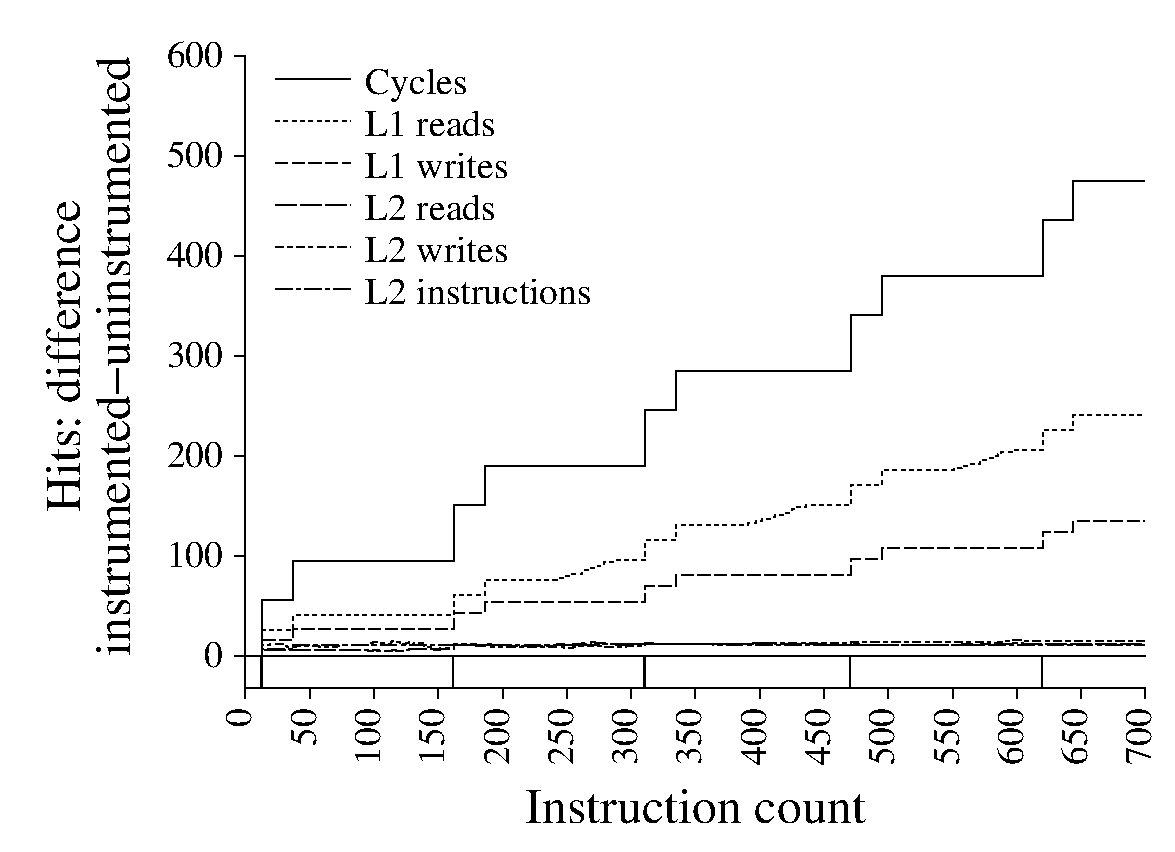
\epsfig{height=0.38\linewidth, file=data/lopi/eps/hits_183.equake_inso_exact} &
    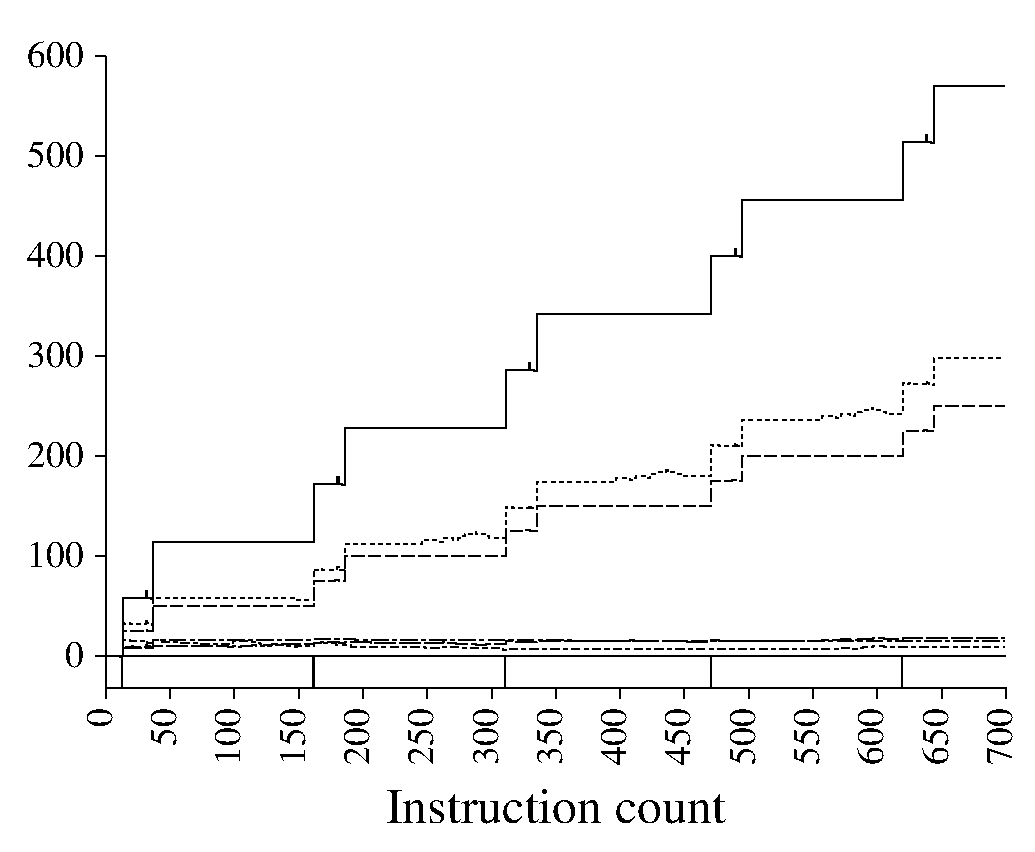
\epsfig{height=0.38\linewidth, file=data/lopi/eps/hits_183.equake_dyninst_exact} \\
    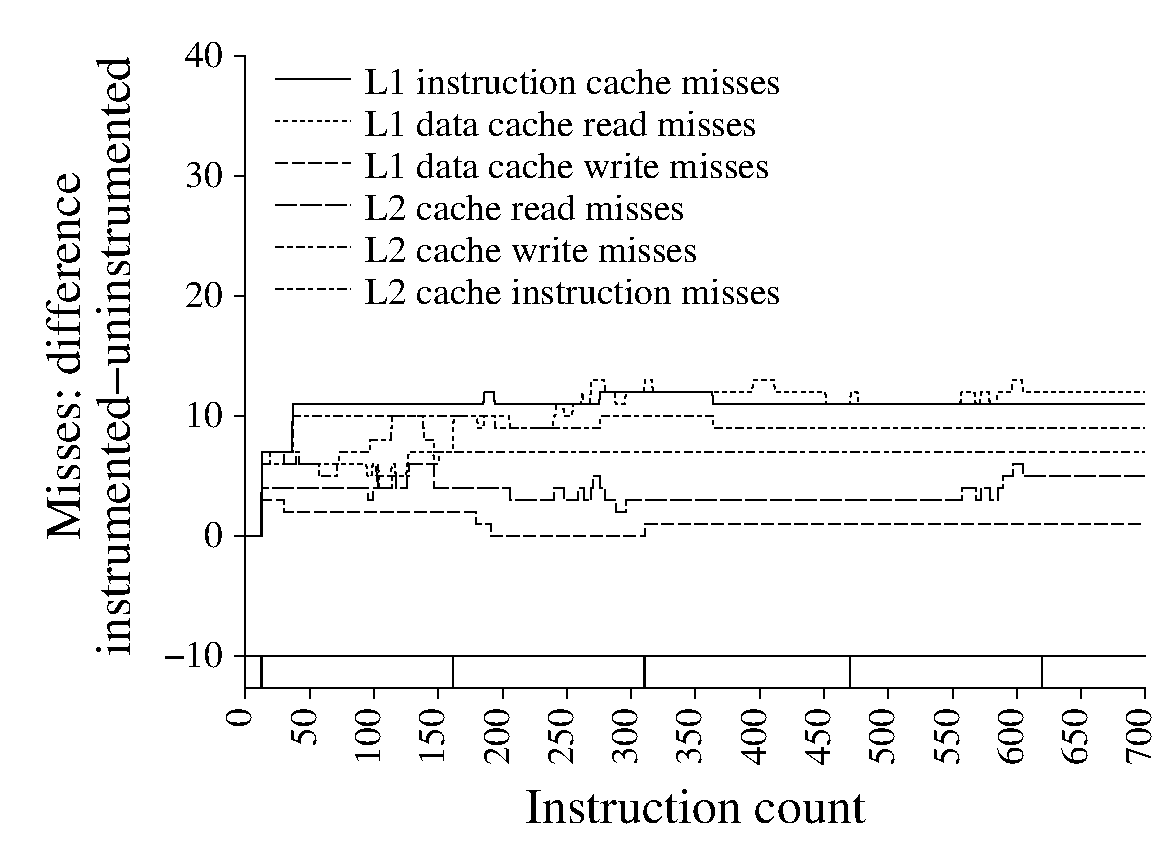
\epsfig{height=0.38\linewidth, file=data/lopi/eps/misses_183.equake_inso_exact} &
    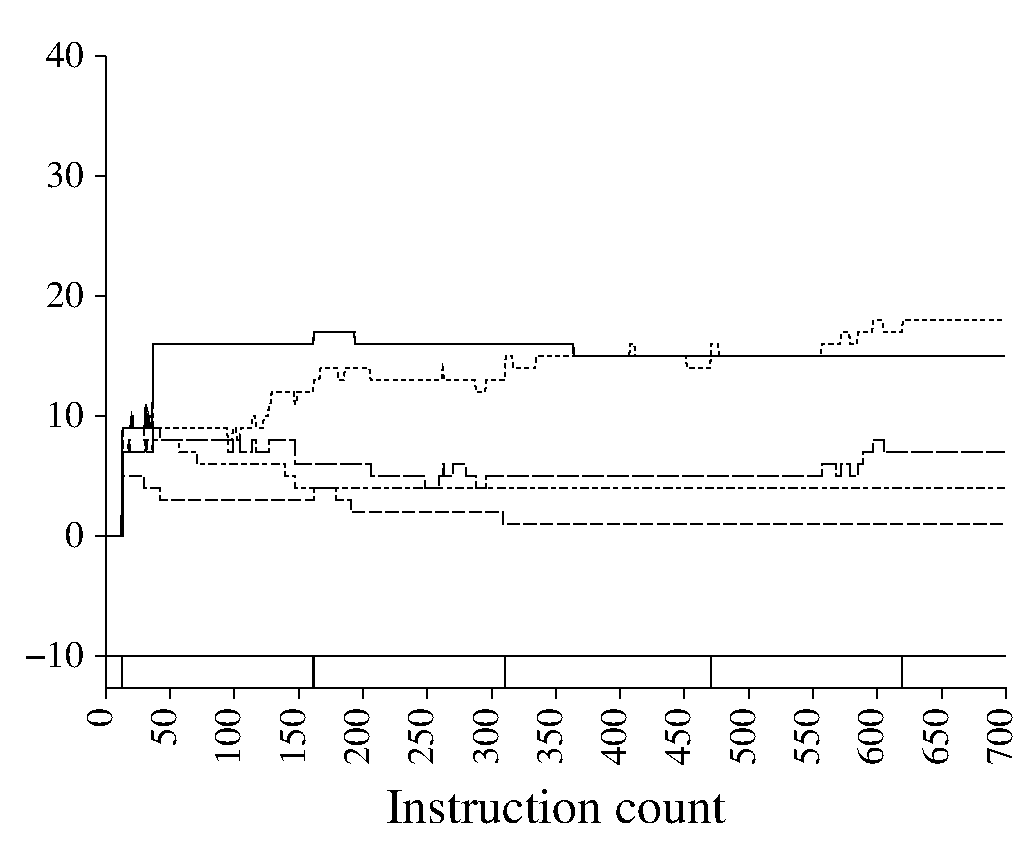
\epsfig{height=0.38\linewidth, file=data/lopi/eps/misses_183.equake_dyninst_exact} \\
  \end{array}$
  \caption[Execution profile for two SPEC benchmarks.]{\emph{Continued on next
    page.}}
  \label{fig:lopi:exec_profile}
\end{figure*}
\begin{figure*}[t!]
  \centering{197.parser}
  $\begin{array}{cc}
    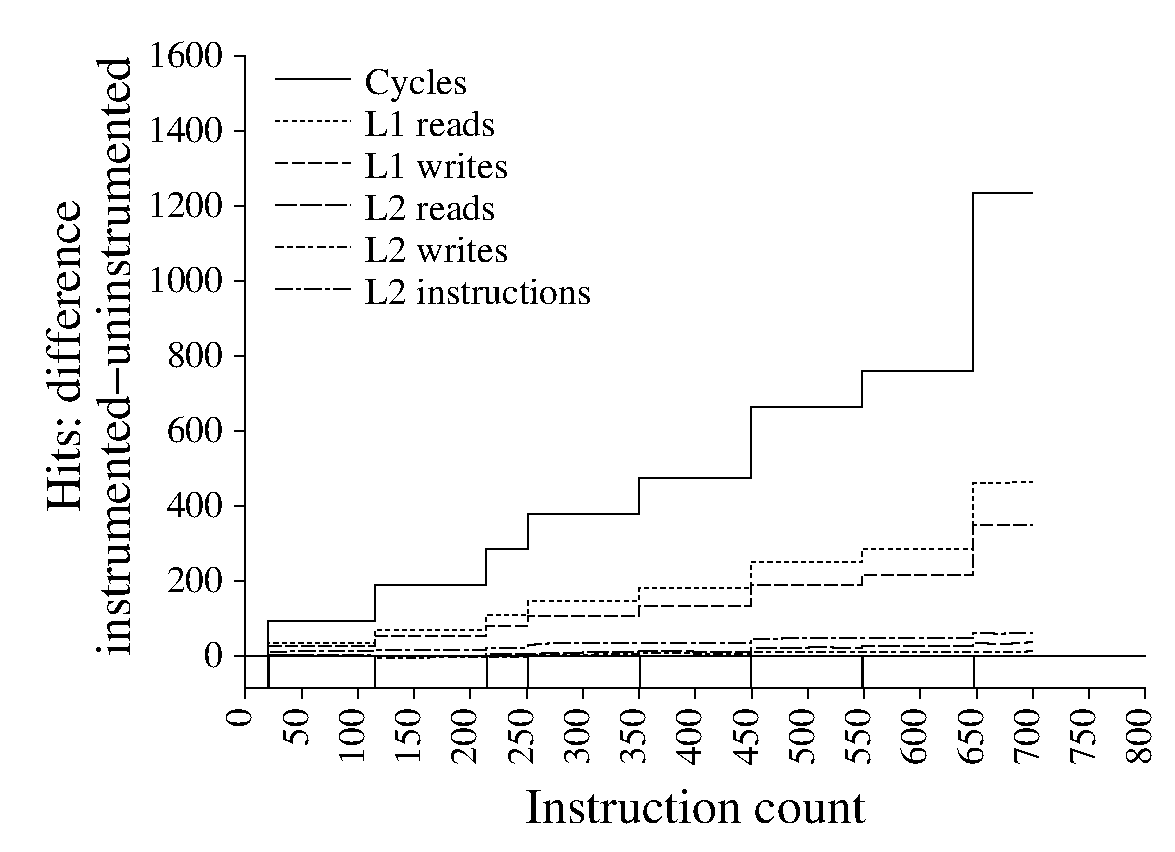
\epsfig{height=0.38\linewidth, file=data/lopi/eps/hits_197.parser_inso_exact} &
    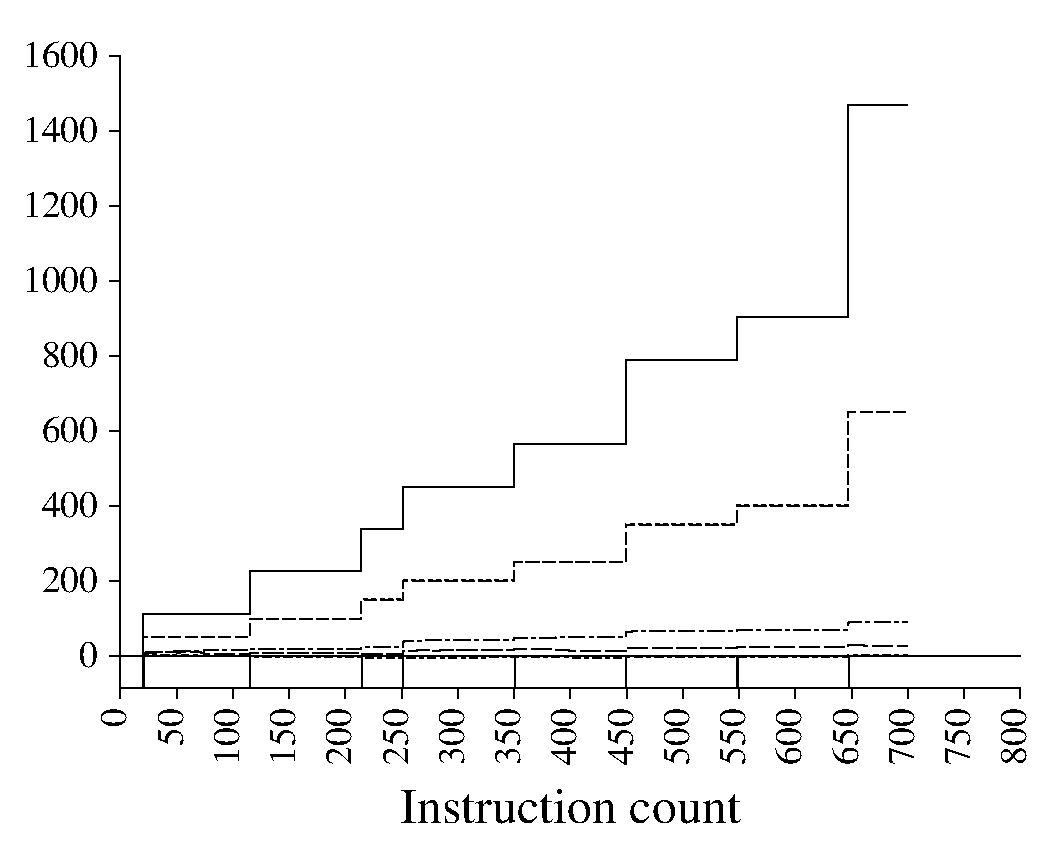
\epsfig{height=0.38\linewidth, file=data/lopi/eps/hits_197.parser_dyninst_exact} \\
    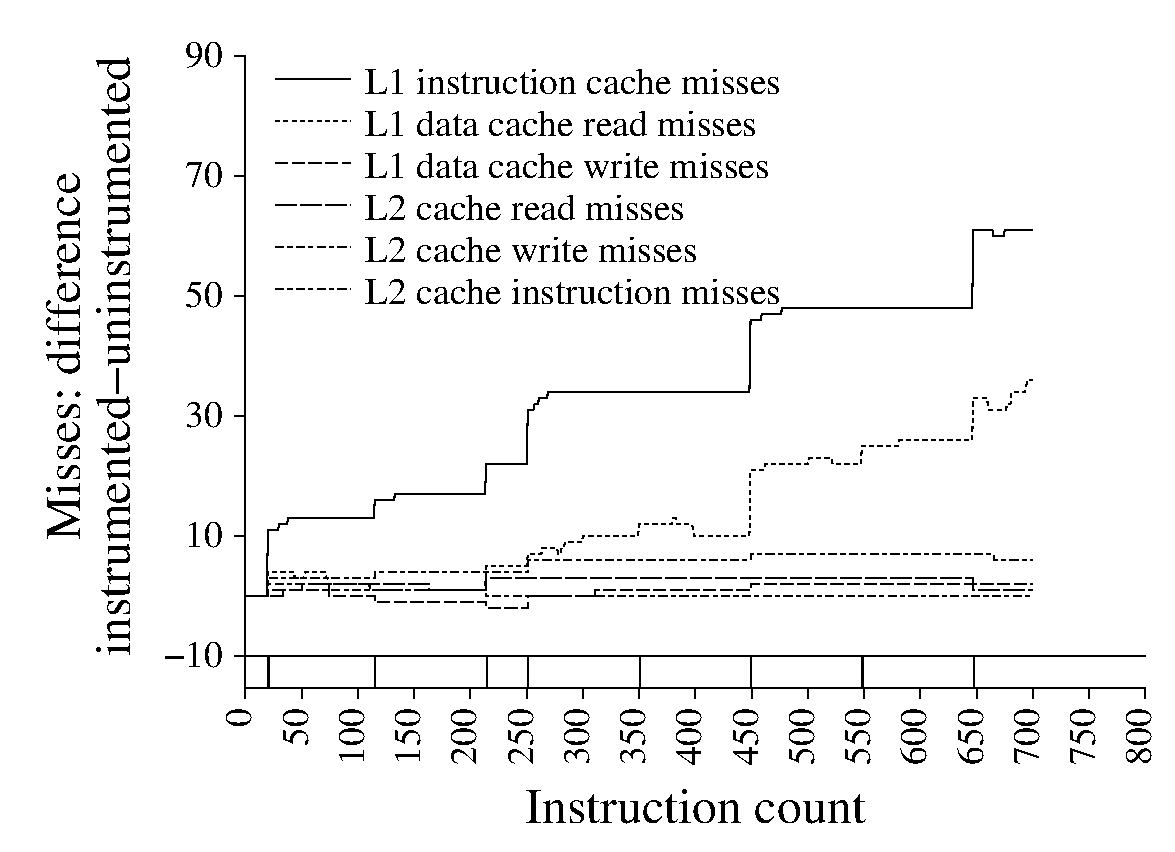
\epsfig{height=0.38\linewidth, file=data/lopi/eps/misses_197.parser_inso_exact} &
    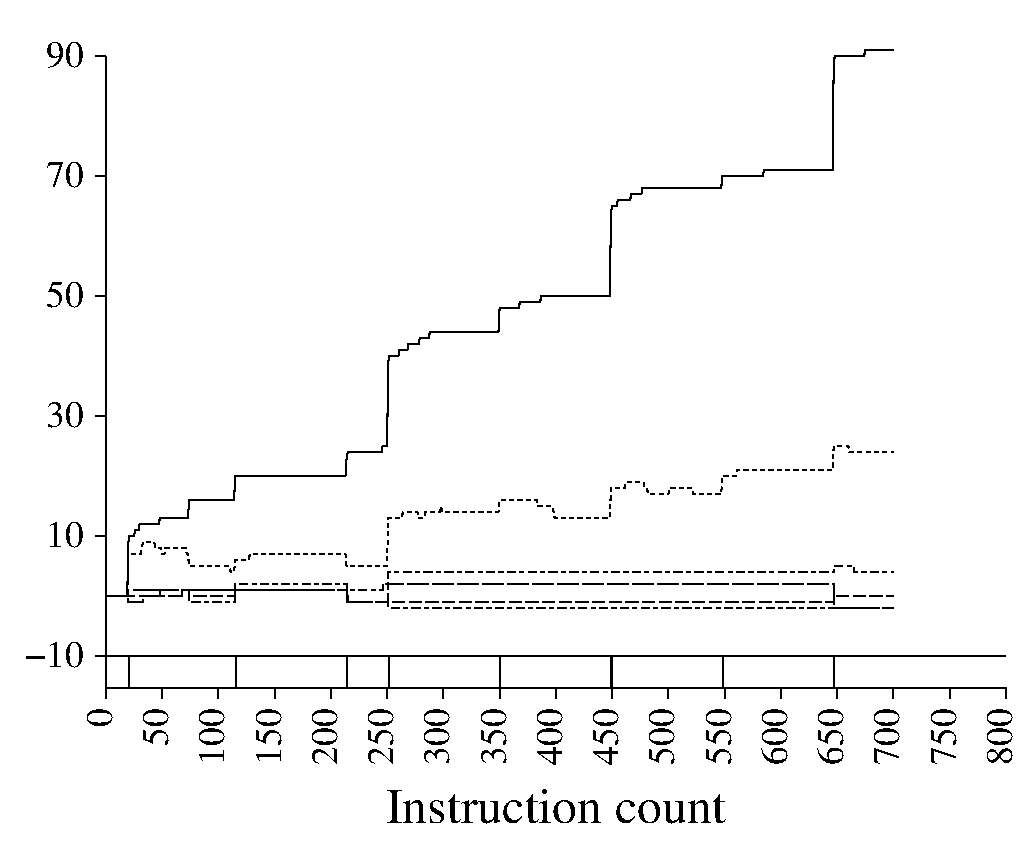
\epsfig{height=0.38\linewidth, file=data/lopi/eps/misses_197.parser_dyninst_exact} \\
  \end{array}$
  \begin{flushleft}
    Figure~\ref{fig:lopi:exec_profile}: Partial execution
    profile for 183.equake and 197.parser. LOPI is shown on the left, Dyninst
    on the right.
  \end{flushleft}
\end{figure*}

Analyzing the cache misses we find that LOPI generates fewer first level cache
accesses on average than Dyninst does, but LOPI has more first-level cache
misses than Dyninst. This indicates a higher locality in the Dyninst code.
However, when we look at the second-level cache accesses we find that the
number of misses is comparable for LOPI and Dyninst.  One reason for the
higher number of data read misses for LOPI is that the return frames (which
are logically code) are allocated as data.

We have identified one performance limitation for LOPI~-- a high number of
miss-predicted branches. The Pentium III employs a branch predictor for
function returns, which work as long as functions are called in the ``normal''~
manner, i.e., through a \texttt{call}/\texttt{ret} pair. Since LOPI overwrites
the return address with an address in the return frame, the return branch
predictor misses its prediction, resulting in a performance loss. This problem
was not visible in the simulated results.

Figure~\ref{fig:lopi:exec_profile} presents a partial execution profile for the
183.equake and 197.parser SPEC benchmarks.  The figure shows the difference
between an instrumented and a non-instrumented run for both LOPI and Dyninst
(note that the graph does not show the absolute values, which start at higher
than zero).  The profiles are constructed from a trace of every instruction in
the shown code snippet (except for the instrumentation code), i.e., every
point in time in the figure corresponds to one instruction in the
non-instrumented code.  Instrumentation points for function entries are shown
as vertical bars below the x-axis.

The 183.equake profile comes from the execution of a nested execution loop,
which calls three short functions \emph{phi0}, \emph{phi1}, and \emph{phi2}
where \emph{phi2} is instrumented. For the 197.parser profile, the
instrumented section shows a section with numerous recursive function calls.
As the Figure shows, the return frames cause some pressure on the caches when
the frames cannot be reused on deeper levels of function nesting (because of
the recursion). This is especially visible for L1 read misses that increase
with each additional instrumented call in Figure~\ref{fig:lopi:exec_profile}.

From the graphs, we can see that the Dyninst instrumentation is more intrusive
than our instrumentation. Our instrumentation is mainly cheaper when
instrumenting the function returns (shown as the second climb in the upper
graphs), which shows that the lazy return instrumentation pays off. We can also
see that the number of cache misses is somewhat higher for Dyninst, although
both instrumentation packages primarily cause cache misses on the first
invocation.
% Comment side effects?


\section{Related work}

\label{sec:lopi:related_work}
In this section we discuss some other tools that are similar to our
instrumentation framework. We start with those that rewrite binary files in
order to instrument an application. Examples of such tools are
PatchWrx~\cite{casmira98tcw}, Etch~\cite{etch}, ATOM~\cite{atom}, and
EEL~\cite{eel}. We thereafter discuss Dyninst~\cite{buck00dyninst, paradyn95},
which rewrites the memory image in order to instrument an application.

PatchWrx, ATOM, and EEL works on RISC processors, where it is easier to
rewrite and patch a binary file since all instructions have the same size. In
order to patch and trace an instruction, you simply replace the traced
instruction with a branch instruction to a code snippet where the replaced
instruction together with the instrumentation code reside. In contrast,
rewriting a binary file for an IA-32-processor is much harder due to variable
instruction length. Etch and LOPI both works for IA-32-binaries, and Dyninst
is available for both RISC and CISC processors.

PatchWrx~\cite{casmira98tcw} is developed for Alpha processors and Windows
NT. PatchWrx utilizes the PALcode on the Alpha processor to capture traces,
and it can patch, i.e., instrument, Windows NT application and system binary
images. PatchWrx replaces all types of branching instructions with
unconditional branches to a patch section where the instrumentation code
reside. PatchWrx can also trace loads and stores by replacing the load or
store instruction with an unconditional branch to the instrumentation code,
where also the replaced load or store resides.

ATOM~\cite{atom} is developed for Alpha processors and works under Tru64 UNIX.
ATOM is a general framework for building a range of program analysis tools,
e.g., block counting, profiling, and cache simulation. ATOM allows a procedure
call to be inserted before and after any procedure, basic block, or
instruction. The user indicates where the instrumentation points are, and
provides analysis routines that are called at the instrumentation points.
ATOM then builds an instrumented version of the application including the
analysis routines.

EEL~\cite{eel} (Executable Editing Library) is a library for building tools to
analyze and modify executable files. It can be used, e.g., for program
profiling and tracing, cache simulation, and program optimization. EEL runs on
SPARC processors under Solaris, and provides a mostly architecture- and
system-independent set of operations to read, analyze and modify code in an
executable file.  The user can provide code snippets that can be inserted at
arbitrary places in the binary code. EEL is capable of sophisticated code
analysis, e.g., control-flow graph analysis and live/dead register analysis.

Etch~\cite{etch} is a general-purpose tool for rewriting Win32 binaries for
IA-32-processors. Etch provides a framework for handling the complexities of
both the Win32 executable format as well as the IA-32 instruction set. Important
issues with the Win32 format that Etch solves are to correctly identify code
and data sections, as well as identification of all dynamically loaded
libraries and modules. Etch can be used, e.g., for tracing all loads and
stores, measuring instruction mixes, and code transformation for performance
improvements.  There is also a graphical user interface provided with Etch.

Dyninst~\cite{buck00dyninst, paradyn95} patches and instruments the application
in-core, i.e., after the program has been loaded into memory.  This approach
allows instrumentation to be added to and removed from the program during
runtime. For example, instrumentation can be added where new hot-spots in the
code are detected during runtime, and instrumentation can be dynamically
removed when it is no longer needed, which can reduce unnecessary overhead.
Memory image rewriting also opens up the possibility to instrument operating
system kernels~\cite{tamches1999kerninst}, which cannot be restarted in order
to have the instrumentation take effect.

Pin~\cite{luk05pin,Pinpoint} is a tool for dynamic instrumentation of Linux
applications available for IA-32e, ARM, Itanium and IA-32e. It provides an API
for inserting function calls to user-defined measurement functions at
arbitrary points in the code. Pin performs the program instrumentation at run
time, using a just-in time compiler to instrument and translate the
application.  As a result, Pin can handle shared libraries, multi-threaded
applications, as well as mixed code and data.
% FIXME: Check similarities between Valgrind and pin

\section{Conclusions}
\label{sec:lopi:conclusion}

Program instrumentation is an important technique in many areas, e.g.,
performance measurements, debugging, and coverage analysis.  To be useful,
instrumentation must be easy to apply and it should perturb the application
execution as little as possible. In this paper we present and evaluate the
LOPI framework, which provides a low-overhead generic solution to program
instrumentation.  The LOPI framework automatically instruments an application
by rewriting the binary file(s) by adding one step in the compilation process.
LOPI gives low overhead by applying techniques to reduce the number of added
instructions to the program and by using a lazy method for instrumenting
function returns.

We provide detailed measurements of the instrumentation perturbation using
hardware and full-system simulations of seven SPEC CPU2000 benchmarks. We
compare the LOPI framework to the state-of-the-art Dyninst package and regular
source-based instrumentation.  The measurements show that source-based
instrumentation has the lowest instruction overhead, on average 13\%, but
requires significantly more tedious work for instrumenting the code.
Comparing LOPI and Dyninst we find that LOPI has lower instruction overhead
than Dyninst, on average 36\% as compared to 49\%, respectively. In terms of
execution time, LOPI increases the execution time by 22\% compared to
uninstrumented operation whereas Dyninst adds 28\%.

% FIXME: Add discussion about code splicing here
We believe that the LOPI framework is a viable and flexible way for automatic
program instrumentation with low perturbation. Future work on LOPI involves
adding support for instrumentation at arbitrary program locations, which would
require copying overwritten instruction into the entry stub and saving live
registers at the instrumentation point. Like Dyninst does, this would require
careful handling of replacing instructions, especially on architectures with
variable-length instructions. Another possibility is to port the framework to
other architectures than IA-32, which could require other optimizations than
those explored here.

\section*{Availability}
\noindent
LOPI is available as free software licensed under the GNU GPL at
\url{http://www.ipd.bth.se/ska/lopi.html}.
